Multi-task learning has recently gained in popularity in machine learning after the success in many different domains such as speech recognition~\cite{deng2013new}, computer vision~\cite{girshick2015fast}, natural language processing~\cite{collobert2008unified}, and drug discovery~\cite{ramsundar2015massively}. It aims at leveraging information from relevant tasks in order to improve the generalisation performance in all tasks. Multi-task learning tries to mimic the way people learn, that is, by transferring knowledge from one task to another when the tasks are related. So it is useful to learn multiple tasks simultaneously since the knowledge from one task can be utilised in the other task.

Multi-task learning is related to other areas of machine learning including transfer-learning described on chapter~\ref{ch:transfer learning}. The main difference between those two techniques is that in transfer-learning, the transfer of knowledge between related tasks is done sequentially, and the main goal is to improve the performance of the target task, while in multi-task learning the learning process is parallel for all tasks and the goal is to improve the performance for all tasks. Generally the goal of multi-task learning is to improve the generalisation performance for all related tasks. There are two ways to perform multi-task learning in deep networks. In the context of Deep learning, multi-task learning is done with either hard or soft parameter sharing of the layers.

\begin{figure}[H]
    \begin{center}
    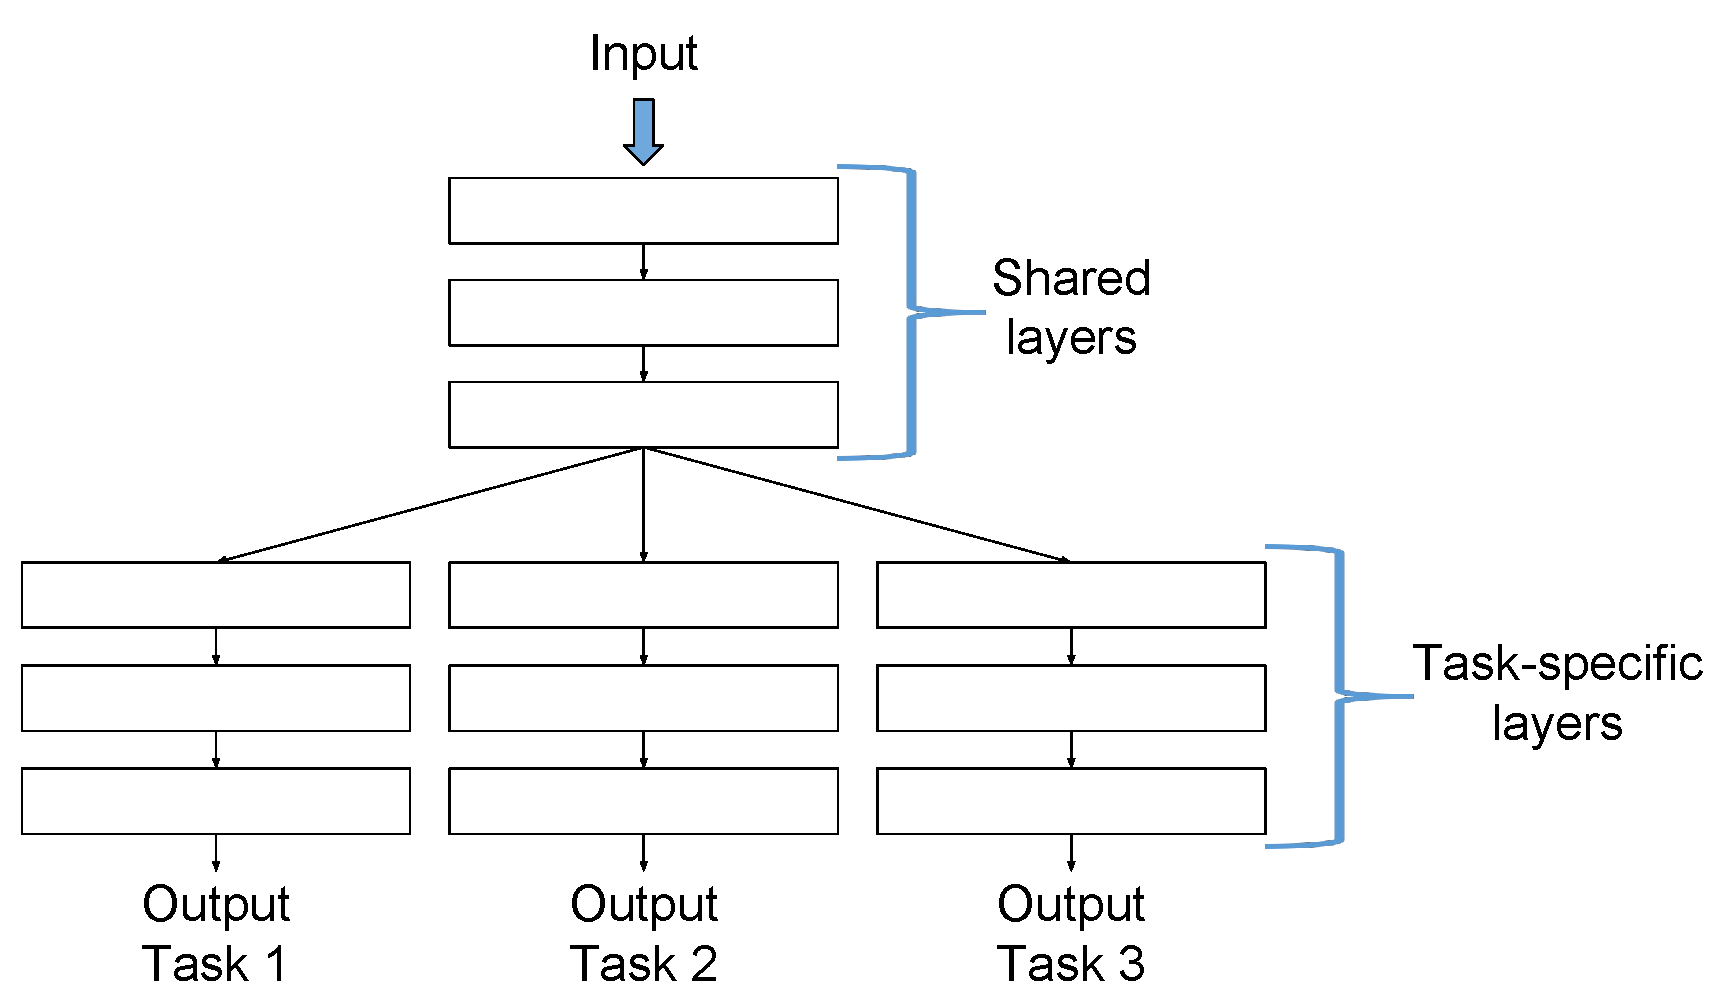
\includegraphics[width=0.8\textwidth]{images/multitask_learning_hard.pdf}
    \end{center}
    \caption{Hard parameter sharing for multi-task learning in deep neural networks} \label{fig:multitask_learning_hard}
\end{figure}

\section{Hard parameter sharing}
Hard parameter sharing~\cite{caruanamultitask} is applied by sharing some layers between all tasks and keeping some task-specific layers for each task as depicted in Figure~\ref{fig:multitask_learning_hard}.It is by far the most commonly used approach to multi-task learning. This approach reduces the risk of overfitting because it tries to find a common representation that works well for all tasks.


\section{Soft parameter sharing}
In soft parameter sharing each task has its own set of parameters and its own model. The distance between the parameters of each task is then regularized for example by using $\ell$2 norm as~\cite{duong2015low} in order to force the parameters to be as similar as possible.  

\begin{figure}[H]
    \begin{center}
    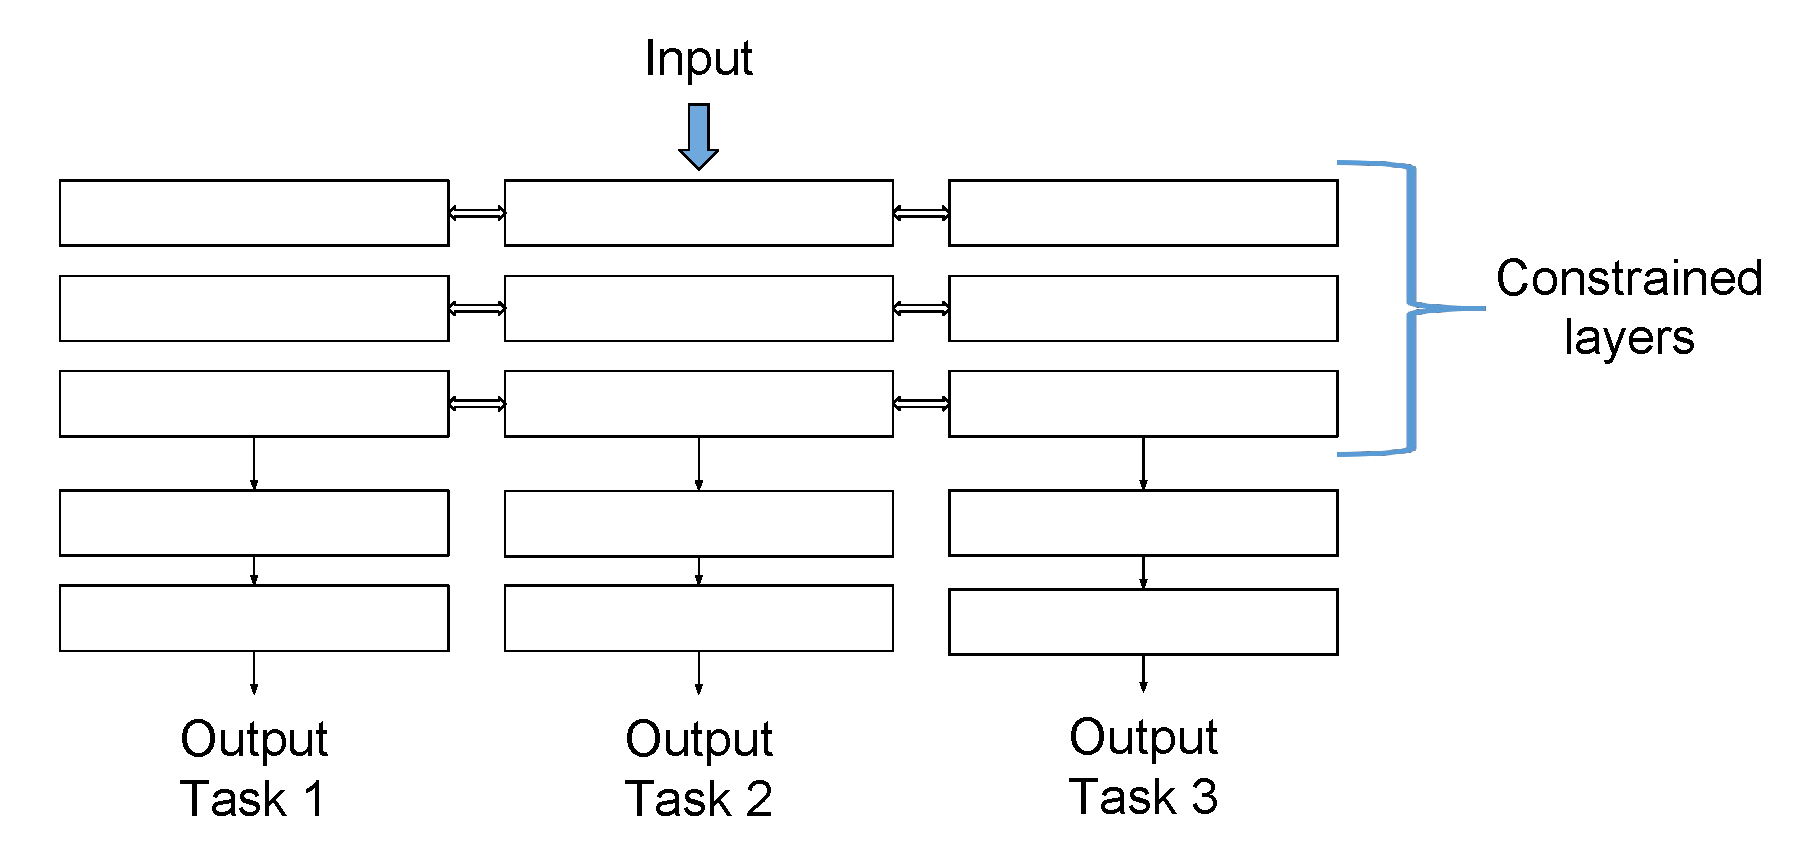
\includegraphics[width=0.8\textwidth]{images/multitask_learning_soft.pdf}
    \end{center}
    \caption{Soft parameter sharing for multi-task learning in deep neural networks} \label{fig:multitask_learning_soft}
\end{figure}

% \afterpage{\blankpage}